\documentclass{standalone}
\usepackage{tikz}
\usetikzlibrary{patterns, positioning}


\begin{document}
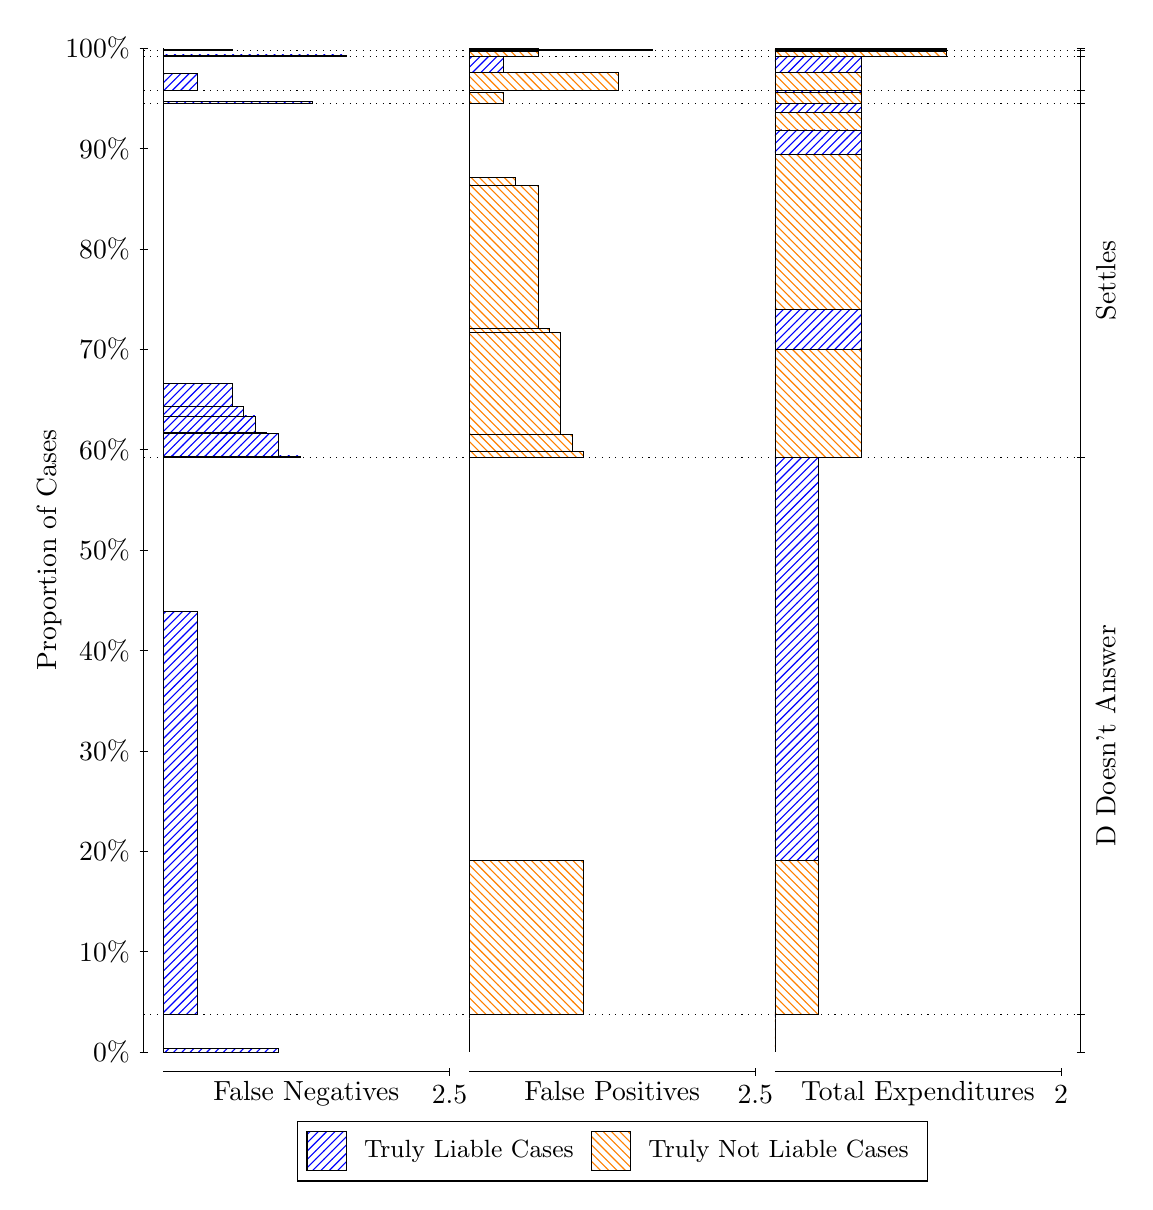
\begin{tikzpicture}
\draw[black, very thin] (1.5,1.75) -- (1.5,14.5);
\node[rotate=90, text=black, anchor=center] at (0.3, 8.125) {Proportion of Cases};
\draw[black, very thin] (1.45,1.75) -- (1.55,1.75);
\node[text=black, anchor=east] at (1.45, 1.75) {0\%};
\draw[black, very thin] (1.45,3.025) -- (1.55,3.025);
\node[text=black, anchor=east] at (1.45, 3.025) {10\%};
\draw[black, very thin] (1.45,4.3) -- (1.55,4.3);
\node[text=black, anchor=east] at (1.45, 4.3) {20\%};
\draw[black, very thin] (1.45,5.575) -- (1.55,5.575);
\node[text=black, anchor=east] at (1.45, 5.575) {30\%};
\draw[black, very thin] (1.45,6.85) -- (1.55,6.85);
\node[text=black, anchor=east] at (1.45, 6.85) {40\%};
\draw[black, very thin] (1.45,8.125) -- (1.55,8.125);
\node[text=black, anchor=east] at (1.45, 8.125) {50\%};
\draw[black, very thin] (1.45,9.4) -- (1.55,9.4);
\node[text=black, anchor=east] at (1.45, 9.4) {60\%};
\draw[black, very thin] (1.45,10.675) -- (1.55,10.675);
\node[text=black, anchor=east] at (1.45, 10.675) {70\%};
\draw[black, very thin] (1.45,11.95) -- (1.55,11.95);
\node[text=black, anchor=east] at (1.45, 11.95) {80\%};
\draw[black, very thin] (1.45,13.225) -- (1.55,13.225);
\node[text=black, anchor=east] at (1.45, 13.225) {90\%};
\draw[black, very thin] (1.45,14.5) -- (1.55,14.5);
\node[text=black, anchor=east] at (1.45, 14.5) {100\%};

\draw[black, very thin] (13.4,1.75) -- (13.4,14.5);
\draw[black, very thin] (13.35,1.75) -- (13.45,1.75);
\node[anchor=west] at (13.35, 1.75) {};
\draw[black, very thin] (13.35,2.2245) -- (13.45,2.2245);
\node[anchor=west] at (13.35, 2.2245) {};
\draw[black, very thin] (13.35,9.3025) -- (13.45,9.3025);
\node[anchor=west] at (13.35, 9.3025) {};
\draw[black, very thin] (13.35,13.799) -- (13.45,13.799);
\node[anchor=west] at (13.35, 13.799) {};
\draw[black, very thin] (13.35,13.964) -- (13.45,13.964);
\node[anchor=west] at (13.35, 13.964) {};
\draw[black, very thin] (13.35,14.398) -- (13.45,14.398);
\node[anchor=west] at (13.35, 14.398) {};
\draw[black, very thin] (13.35,14.469) -- (13.45,14.469);
\node[anchor=west] at (13.35, 14.469) {};
\draw[black, very thin] (13.35,14.5) -- (13.45,14.5);
\node[anchor=west] at (13.35, 14.5) {};

\draw[black, very thin, pattern color=blue, pattern=north east lines] (1.75,1.75) rectangle (3.2033,1.7999);
\draw[black, very thin, pattern color=orange, pattern=north west lines] (1.75,1.7999) rectangle (1.75,2.2245);
\draw[black, very thin, pattern color=blue, pattern=north east lines] (1.75,2.2245) rectangle (2.186,7.3422);
\draw[black, very thin, pattern color=orange, pattern=north west lines] (1.75,7.3422) rectangle (1.75,9.3025);
\draw[black, very thin, pattern color=blue, pattern=north east lines] (1.75,9.3025) rectangle (3.494,9.3192);
\draw[black, very thin, pattern color=blue, pattern=north east lines] (1.75,9.3192) rectangle (3.2033,9.6028);
\draw[black, very thin, pattern color=blue, pattern=north east lines] (1.75,9.6028) rectangle (3.058,9.6141);
\draw[black, very thin, pattern color=blue, pattern=north east lines] (1.75,9.6141) rectangle (2.9127,9.8281);
\draw[black, very thin, pattern color=blue, pattern=north east lines] (1.75,9.8281) rectangle (2.7673,9.9473);
\draw[black, very thin, pattern color=blue, pattern=north east lines] (1.75,9.9473) rectangle (2.622,10.243);
\draw[black, very thin, pattern color=orange, pattern=north west lines] (1.75,10.243) rectangle (1.75,13.799);
\draw[black, very thin, pattern color=blue, pattern=north east lines] (1.75,13.799) rectangle (3.6393,13.823);
\draw[black, very thin, pattern color=orange, pattern=north west lines] (1.75,13.823) rectangle (1.75,13.964);
\draw[black, very thin, pattern color=blue, pattern=north east lines] (1.75,13.964) rectangle (2.186,14.176);
\draw[black, very thin, pattern color=orange, pattern=north west lines] (1.75,14.176) rectangle (1.75,14.398);
\draw[black, very thin, pattern color=blue, pattern=north east lines] (1.75,14.398) rectangle (4.0753,14.414);
\draw[black, very thin, pattern color=orange, pattern=north west lines] (1.75,14.414) rectangle (1.75,14.469);
\draw[black, very thin, pattern color=blue, pattern=north east lines] (1.75,14.469) rectangle (2.622,14.484);
\draw[black, very thin, pattern color=orange, pattern=north west lines] (1.75,14.484) rectangle (1.75,14.5);
\draw[black, very thin, pattern color=orange, pattern=north west lines] (5.6333,1.75) rectangle (5.6333,2.1746);
\draw[black, very thin, pattern color=blue, pattern=north east lines] (5.6333,2.1746) rectangle (5.6333,2.2245);
\draw[black, very thin, pattern color=orange, pattern=north west lines] (5.6333,2.2245) rectangle (7.0867,4.1848);
\draw[black, very thin, pattern color=blue, pattern=north east lines] (5.6333,4.1848) rectangle (5.6333,9.3025);
\draw[black, very thin, pattern color=orange, pattern=north west lines] (5.6333,9.3025) rectangle (7.0867,9.3748);
\draw[black, very thin, pattern color=orange, pattern=north west lines] (5.6333,9.3748) rectangle (6.9413,9.5957);
\draw[black, very thin, pattern color=orange, pattern=north west lines] (5.6333,9.5957) rectangle (6.796,10.893);
\draw[black, very thin, pattern color=orange, pattern=north west lines] (5.6333,10.893) rectangle (6.6507,10.935);
\draw[black, very thin, pattern color=orange, pattern=north west lines] (5.6333,10.935) rectangle (6.5053,12.755);
\draw[black, very thin, pattern color=orange, pattern=north west lines] (5.6333,12.755) rectangle (6.2147,12.859);
\draw[black, very thin, pattern color=blue, pattern=north east lines] (5.6333,12.859) rectangle (5.6333,13.799);
\draw[black, very thin, pattern color=orange, pattern=north west lines] (5.6333,13.799) rectangle (6.0693,13.94);
\draw[black, very thin, pattern color=blue, pattern=north east lines] (5.6333,13.94) rectangle (5.6333,13.964);
\draw[black, very thin, pattern color=orange, pattern=north west lines] (5.6333,13.964) rectangle (7.5227,14.186);
\draw[black, very thin, pattern color=blue, pattern=north east lines] (5.6333,14.186) rectangle (6.0693,14.398);
\draw[black, very thin, pattern color=orange, pattern=north west lines] (5.6333,14.398) rectangle (6.5053,14.453);
\draw[black, very thin, pattern color=blue, pattern=north east lines] (5.6333,14.453) rectangle (5.6333,14.469);
\draw[black, very thin, pattern color=orange, pattern=north west lines] (5.6333,14.469) rectangle (7.9587,14.484);
\draw[black, very thin, pattern color=blue, pattern=north east lines] (5.6333,14.484) rectangle (6.5053,14.5);
\draw[black, very thin, pattern color=orange, pattern=north west lines] (9.5167,1.75) rectangle (9.5167,2.1746);
\draw[black, very thin, pattern color=blue, pattern=north east lines] (9.5167,2.1746) rectangle (9.5167,2.2245);
\draw[black, very thin, pattern color=orange, pattern=north west lines] (9.5167,2.2245) rectangle (10.062,4.1848);
\draw[black, very thin, pattern color=blue, pattern=north east lines] (9.5167,4.1848) rectangle (10.062,9.3025);
\draw[black, very thin, pattern color=orange, pattern=north west lines] (9.5167,9.3025) rectangle (10.607,10.672);
\draw[black, very thin, pattern color=blue, pattern=north east lines] (9.5167,10.672) rectangle (10.607,11.182);
\draw[black, very thin, pattern color=orange, pattern=north west lines] (9.5167,11.182) rectangle (10.607,13.147);
\draw[black, very thin, pattern color=blue, pattern=north east lines] (9.5167,13.147) rectangle (10.607,13.459);
\draw[black, very thin, pattern color=orange, pattern=north west lines] (9.5167,13.459) rectangle (10.607,13.68);
\draw[black, very thin, pattern color=blue, pattern=north east lines] (9.5167,13.68) rectangle (10.607,13.799);
\draw[black, very thin, pattern color=orange, pattern=north west lines] (9.5167,13.799) rectangle (10.607,13.94);
\draw[black, very thin, pattern color=blue, pattern=north east lines] (9.5167,13.94) rectangle (10.607,13.964);
\draw[black, very thin, pattern color=orange, pattern=north west lines] (9.5167,13.964) rectangle (10.607,14.186);
\draw[black, very thin, pattern color=blue, pattern=north east lines] (9.5167,14.186) rectangle (10.607,14.398);
\draw[black, very thin, pattern color=orange, pattern=north west lines] (9.5167,14.398) rectangle (11.697,14.453);
\draw[black, very thin, pattern color=blue, pattern=north east lines] (9.5167,14.453) rectangle (11.697,14.469);
\draw[black, very thin, pattern color=orange, pattern=north west lines] (9.5167,14.469) rectangle (11.697,14.484);
\draw[black, very thin, pattern color=blue, pattern=north east lines] (9.5167,14.484) rectangle (11.697,14.5);
\draw[black, dotted] (1.5,2.2245) -- (13.4,2.2245);
\draw[black, dotted] (1.5,9.3025) -- (13.4,9.3025);
\draw[black, dotted] (1.5,13.799) -- (13.4,13.799);
\draw[black, dotted] (1.5,13.964) -- (13.4,13.964);
\draw[black, dotted] (1.5,14.398) -- (13.4,14.398);
\draw[black, dotted] (1.5,14.469) -- (13.4,14.469);
\draw[black, very thin] (1.75,1.5) -- (5.3833,1.5);
\node[text=black, anchor=north] at (3.5667, 1.5) {False Negatives};
\draw[black, very thin] (5.3833,1.45) -- (5.3833,1.55);
\node[text=black, anchor=north] at (5.3833, 1.45) {2.5};

\draw[black, very thin] (5.6333,1.5) -- (9.2667,1.5);
\node[text=black, anchor=north] at (7.45, 1.5) {False Positives};
\draw[black, very thin] (9.2667,1.45) -- (9.2667,1.55);
\node[text=black, anchor=north] at (9.2667, 1.45) {2.5};

\draw[black, very thin] (9.5167,1.5) -- (13.15,1.5);
\node[text=black, anchor=north] at (11.333, 1.5) {Total Expenditures};
\draw[black, very thin] (13.15,1.45) -- (13.15,1.55);
\node[text=black, anchor=north] at (13.15, 1.45) {2};


\node[text=black, centered, rotate=90] at (13.72, 5.7635) {D Doesn't Answer};
\node[text=black, centered, rotate=90] at (13.72, 11.551) {Settles};





\draw (7.449999999999999,1.5) node[draw=none] (baseCoordinate) {};
\begin{scope}[align=center]
        \matrix[scale=0.5, draw=black, below=0.5cm of baseCoordinate, nodes={draw}, column sep=0.1cm]{
            \node[rectangle, draw, minimum width=0.5cm, minimum height=0.5cm, pattern color=blue, pattern=north east lines] {}; &
            \node[draw=none, font=\small, text=black] (B) {Truly Liable Cases}; &
            \node[rectangle, draw, minimum width=0.5cm, minimum height=0.5cm, pattern color=orange, pattern=north west lines] {}; &
            \node[draw=none, font=\small, text=black] (B) {Truly Not Liable Cases}; \\
            };
\end{scope}

\end{tikzpicture}
\end{document}